% Options for packages loaded elsewhere
\PassOptionsToPackage{unicode}{hyperref}
\PassOptionsToPackage{hyphens}{url}
%
\documentclass[
]{article}
\usepackage{amsmath,amssymb}
\usepackage{iftex}
\ifPDFTeX
  \usepackage[T1]{fontenc}
  \usepackage[utf8]{inputenc}
  \usepackage{textcomp} % provide euro and other symbols
\else % if luatex or xetex
  \usepackage{unicode-math} % this also loads fontspec
  \defaultfontfeatures{Scale=MatchLowercase}
  \defaultfontfeatures[\rmfamily]{Ligatures=TeX,Scale=1}
\fi
\usepackage{lmodern}
\ifPDFTeX\else
  % xetex/luatex font selection
\fi
% Use upquote if available, for straight quotes in verbatim environments
\IfFileExists{upquote.sty}{\usepackage{upquote}}{}
\IfFileExists{microtype.sty}{% use microtype if available
  \usepackage[]{microtype}
  \UseMicrotypeSet[protrusion]{basicmath} % disable protrusion for tt fonts
}{}
\makeatletter
\@ifundefined{KOMAClassName}{% if non-KOMA class
  \IfFileExists{parskip.sty}{%
    \usepackage{parskip}
  }{% else
    \setlength{\parindent}{0pt}
    \setlength{\parskip}{6pt plus 2pt minus 1pt}}
}{% if KOMA class
  \KOMAoptions{parskip=half}}
\makeatother
\usepackage{xcolor}
\usepackage[margin=1in]{geometry}
\usepackage{graphicx}
\makeatletter
\def\maxwidth{\ifdim\Gin@nat@width>\linewidth\linewidth\else\Gin@nat@width\fi}
\def\maxheight{\ifdim\Gin@nat@height>\textheight\textheight\else\Gin@nat@height\fi}
\makeatother
% Scale images if necessary, so that they will not overflow the page
% margins by default, and it is still possible to overwrite the defaults
% using explicit options in \includegraphics[width, height, ...]{}
\setkeys{Gin}{width=\maxwidth,height=\maxheight,keepaspectratio}
% Set default figure placement to htbp
\makeatletter
\def\fps@figure{htbp}
\makeatother
\setlength{\emergencystretch}{3em} % prevent overfull lines
\providecommand{\tightlist}{%
  \setlength{\itemsep}{0pt}\setlength{\parskip}{0pt}}
\setcounter{secnumdepth}{-\maxdimen} % remove section numbering
\usepackage{float}
\ifLuaTeX
  \usepackage{selnolig}  % disable illegal ligatures
\fi
\IfFileExists{bookmark.sty}{\usepackage{bookmark}}{\usepackage{hyperref}}
\IfFileExists{xurl.sty}{\usepackage{xurl}}{} % add URL line breaks if available
\urlstyle{same}
\hypersetup{
  pdftitle={Taller de Análisis de datos - Problema de clasificación 0},
  pdfauthor={Jésica Charaf e Ignacio Spiousas},
  hidelinks,
  pdfcreator={LaTeX via pandoc}}

\title{Taller de Análisis de datos - Problema de clasificación 0}
\author{Jésica Charaf e Ignacio Spiousas}
\date{24 de noviembre de 2023}

\begin{document}
\maketitle

\hypertarget{problema-de-clasificaciuxf3n-0}{%
\section{Problema de clasificación
0}\label{problema-de-clasificaciuxf3n-0}}

El archivo Distrofia-info contiene una descripción de la Distrofia
Muscular de Duchenne (DMD), para cuyo diagnóstico se realizó un estudio
cuyos resultados están en el archivo Distrofia-Data. La primera fila es:

\texttt{38\ \ \ 1\ \ \ \ \ 1\ \ \ \ 1\ 1007\ 22\ 6\ 0\ 079\ 52.0\ 83.5\ 10.9\ 176}

Las primeras 5 columnas no sirven. ``22'' es la edad, ``6'' el mes,
``0'' no sirve, ``079'' el año, y las últimas cuatro son CK, H, PK y LD.
El objetivo es proponer una regla para detectar la DMD usando las cuatro
variables observadas (enzimas), y estimar su error de clasificación. Se
plantean algunas preguntas:

\begin{enumerate}
\def\labelenumi{\alph{enumi})}
\item
  CK y H son más baratas de medir que PK y LD. ¿Cuánto aumenta el error
  si se prescinde de estas últimas?
\item
  ¿Tiene sentido incluir la edad entre los predictores?
\item
  La sensibilidad y la especificidad son respectivamente las
  probabilidades de identificar correctamente a sujetos enfermos y
  sanos. ¿Cómo elegir el balance entre ambas?
\item
  Se sabe que la probabilidad de que una mujer sea portadora es 1/3200.
  ¿Tiene alguna utilidad ese dato?
\end{enumerate}

\hypertarget{resoluciuxf3n}{%
\section{Resolución}\label{resoluciuxf3n}}

\hypertarget{anuxe1lisis-exploratorio}{%
\subsection{Análisis exploratorio}\label{anuxe1lisis-exploratorio}}

El conjunto de datos contiene 209 observaciones dentro de las cuales 134
corresponden a la clase no portadora y 75 a la clase portadora. Las
variables involucradas son:

\begin{itemize}
\tightlist
\item
  Edad
\item
  Mes
\item
  Año
\item
  CK
\item
  H
\item
  PK
\item
  LD
\end{itemize}

Para empezar, inspeccionamos los datos y detectamos observaciones con
valores faltantes registrados como ``-9999'' dentro de las variables PK
y LD. Estos valores fueron reemplazados por el promedio por clase de los
valores registrados en cada variable.

En la figura \ref{fig:edades} pueden verse los boxplots de las edades
según cada clase y podemos observar que, aparentemente, no hay
representatividad de edades más grandes en la muestra no portadora, lo
cual parece estar vinculado a cómo se tomó la muestra y no
necesariamente a que haya una relación directa entre la edad y la
pertenencia a alguna de las clases. Esta heterogeneidad podría
enmascarar el efecto de los marcadores en el diagnóstico por la edad y
es por este motivo que no incluiremos esta variable como predictora.

\begin{figure}[H]

{\centering 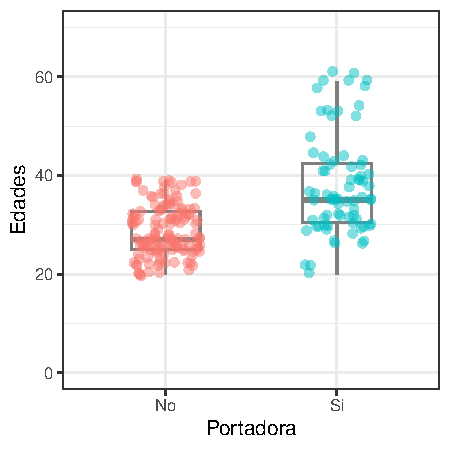
\includegraphics{Charaf-Spiousas_Clasificacion0_files/figure-latex/unnamed-chunk-2-1} 

}

\caption{\label{fig:edades}Boxplots de las edades según la condición de portadora junto con las observaciones individuales.}\label{fig:unnamed-chunk-2}
\end{figure}

Una vez limpiados los datos, consideramos las 4 columnas que indican los
valores detectados de ciertos marcadores (CK, H, PK y LD) y una columna
con los valores ``Sí'' o ``No'' que indica si la persona es portadora o
no.

En la figura \ref{fig:explo1} se observa la medición de cada marcador
dependiendo de si la persona es o no portadora. A simple vista podemos
ver que, en promedio (barra gris), la medición de los cuatro marcadores
es superior cuando la persona es portadora. Sin embargo, pareciera que H
es el que separa menos eficientemente ambos grupos.

\begin{figure}[H]

{\centering 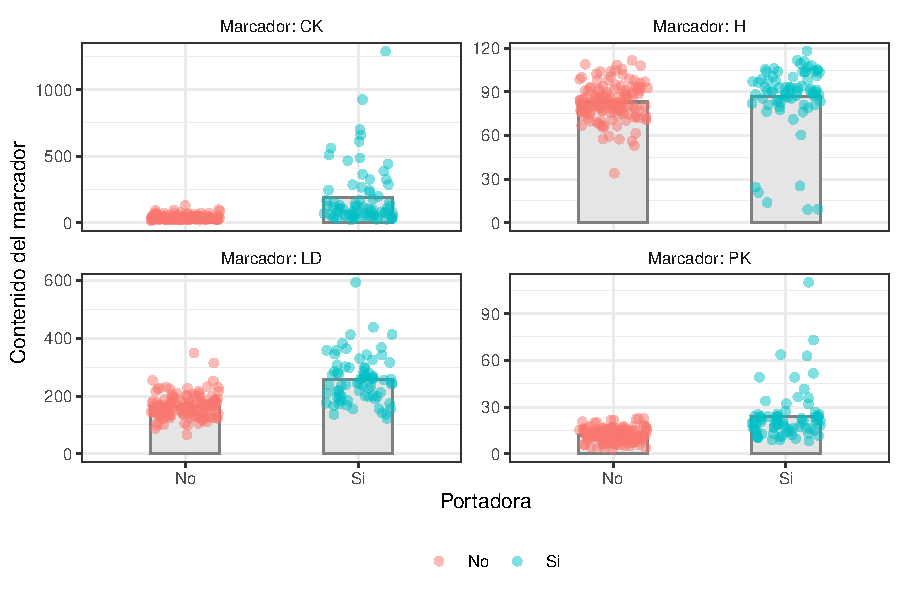
\includegraphics{Charaf-Spiousas_Clasificacion0_files/figure-latex/unnamed-chunk-3-1} 

}

\caption{\label{fig:explo1}Dependencia de la medición de cada marcador con la condición de portadora de la persona. Los puntos indican los datos individuales mientras que la barra gris indica el promedio para cada categoría.}\label{fig:unnamed-chunk-3}
\end{figure}

El objetivo del presente trabajo consiste en entrenar un modelo que
prediga si la persona es portadora o no a partir de las cuatro
mediciones de marcadores. Para esto vamos a evaluar un número de modelos
de clasificación: Regresión logística, K vecinos vercanos y Random
Forest. Luego de elegir qué modelo es el más conveniente para el
problema y ajustar sus hiperparámetros y parámetros evaluaremos su
capacidad de predicción en un set de testeo.

\hypertarget{elecciuxf3n-del-muxe9todo-de-clasificaciuxf3n}{%
\subsection{Elección del método de
clasificación}\label{elecciuxf3n-del-muxe9todo-de-clasificaciuxf3n}}

Para analizar los distintos métodos de clasificación, separamos la
muestra en un set de entrenamiento (dos tercios de los datos) y un set
de testeo (un tercio de los datos) de forma estratificada según la
clase, utilizando la función \texttt{initial\_split} de
\emph{\{rsample\}}.

La métrica a utilizar para evaluar el modelo depende del caso en
particular de estudio y del tipo de error que consideremos que es más
grave cometer o se priorice evitar. En nuestro caso vamos a considerar
la medida \emph{F1 score} teniendo en cuenta que provee un balance entre
\emph{recall} y \emph{precision}.

\hypertarget{k-vecinos-cercanos}{%
\subsubsection{K vecinos cercanos}\label{k-vecinos-cercanos}}

El primer modelo que vamos a ajustar es el de K vecinos cercanos. Para
esto consideramos una grilla de valores de \(k\) (cantidad de vecinos)
entre 1 y 20. Para evaluar cuál es la cantidad de vecinos más
conveniente realizamos validación cruzada separando la muestra de
entrenamiento en 10 folds estratificando según la clase. Estos
\emph{folds} son generados utilizando la función \texttt{vfold\_cv} del
paquete \emph{\{rsample\}}.

Para implementar este modelo utilizaremos las funcionalidades del
paquete \emph{\{tidymodels\}}.

De esta manera, para cada valor de \(k\), calculamos el promedio de los
F1 obtenidos en cada fold y seleccionamos el valor de \(k\) que maximice
dicho promedio. Con este criterio, el valor de \(k\) obtenido es 9 con
un valor de F1 de 0.836. En la figura \ref{fig:knn} podemos ver los
valores promedios de los F1 en función de la cantidad de vecinos
utilizados.

\begin{figure}[H]

{\centering 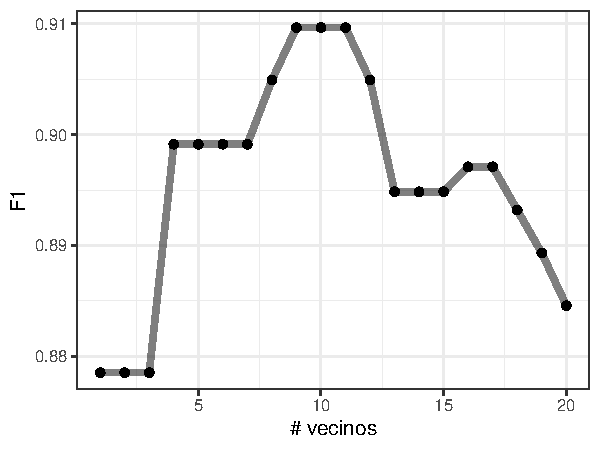
\includegraphics{Charaf-Spiousas_Clasificacion0_files/figure-latex/unnamed-chunk-6-1} 

}

\caption{\label{fig:knn}Dependencia de F1 con la cantidad de vecinos para el modelo de vecinos cercanos.}\label{fig:unnamed-chunk-6}
\end{figure}

\hypertarget{regresiuxf3n-loguxedstica}{%
\subsubsection{Regresión logística}\label{regresiuxf3n-loguxedstica}}

Para continuar, otro enfoque que exploramos es el de regresión logísica
considerando una familia de modelos lineales generalizados con
regularización Lasso.

En este caso, tomamos una grilla de 50 valores de \(\lambda\)
equiespaciados en escala logarítmica entre \(10^{-3}\) y \(10^0\) y, a
la vez, consideramos distintos valores de umbral de clasificación \(p\)
entre 0.2 y 0.8\footnote{Resulta razonable que el óptimo no esté en
  valores muy chicos ni muy grandes.} con paso 0.1.

Al igual que antes, realizamos validación cruzada tomando 10 folds y
evaluando para cada valor de \(\lambda\) y de \(p\) los resultados del
F1 obtenido a partir del ajuste del modelo lineal generalizado
correspondiente asignándole pesos
\(1-\frac{\# \, casos \, de \, la \,clase }{\# \, casos \, totales}\) a
las observaciones correspondientes a cada clase.

El valor máximo obtenido para el F1 es 0.841 y se alcanza para un umbral
de \(p=\) 0.3 y un \(\lambda=\) 0.026827.

\hypertarget{random-forest}{%
\subsubsection{Random forest}\label{random-forest}}

Como última alternativa vamos a considerar un modelo basado en árboles a
partir de la técnica de random forest. En este caso también utilizaremos
validación cruzada para hallar la combinación de parámetros que maximice
F1. Los hiperparámetros sobre los cuales vamos a optimizar son:

\begin{itemize}
\tightlist
\item
  el número de variables que se consideran en cada split del árbol
  aleatorio, que puede tomar valores enteros de 1 a 4 (\texttt{mtry}), y
\item
  el número mínimo de observaciones requeridas para que una hoja se
  bifurque, que puede tomar valores enteros mayores a 1
  (\texttt{min\_n}).
\end{itemize}

De este modo, calcularemos el promedio de los F1 que se obtienen a
partir del ajuste de random forest en los distintos folds para cada
combinación de \texttt{mtry} y \texttt{min\_n} sobre una grilla que
considera valores enteros y rangos \(1 \leq\)\texttt{mtry}\(\leq 4\) y
\(1 \leq\)\texttt{min\_n}\(\leq 40\).

Para implementar este modelo, y al igual que en el caso de K vecinos
cercanos, utilizaremos las funcionalidades del paquete
\emph{\{tidymodels\}}.

\begin{figure}[H]

{\centering 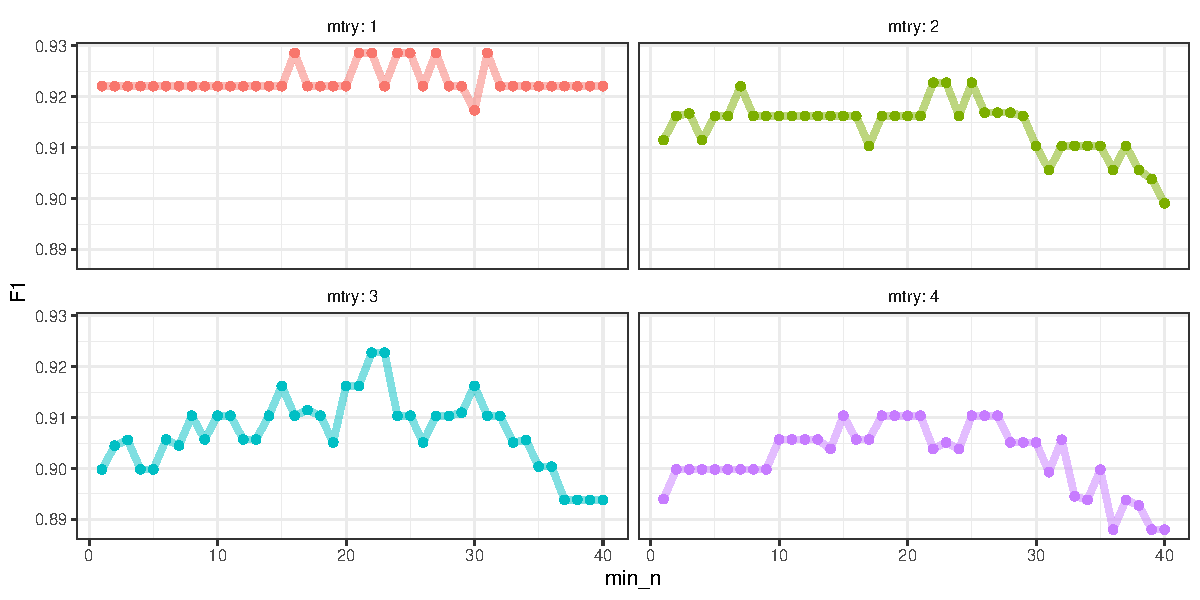
\includegraphics{Charaf-Spiousas_Clasificacion0_files/figure-latex/unnamed-chunk-9-1} 

}

\caption{\label{fig:random}Dependencia del F1 obtenido por validación cruzada con los parámetros de random forest.}\label{fig:unnamed-chunk-9}
\end{figure}

En la figura \ref{fig:random} se pueden ver los resultados del F1 en
función de los parámetros de la grilla. Si bien no pareciera haber una
clara dependencia con \texttt{min\_n}, sí observamos una relación con
\texttt{mtry} donde se obtienen valores de F1 más altos para
\texttt{mtry} igual a 1 y que decrecen para valores más grandes. El
valor máximo obtenido para el F1 es 0.861 y se alcanza para
\texttt{mtry} igual a 1 y \texttt{min\_n} igual a 21.

\hypertarget{evaluaciuxf3n-del-modelo-elegido-en-los-datos-de-testeo}{%
\subsection{\texorpdfstring{Evaluación del modelo elegido en los datos
de
\emph{testeo}}{Evaluación del modelo elegido en los datos de testeo}}\label{evaluaciuxf3n-del-modelo-elegido-en-los-datos-de-testeo}}

En nuestro caso, los mejores modelos de cada tipo tuvieron un desempeño
similar. Es por eso que seleccionaremos el modelo que consideramos más
simple e interpretable, es decir, GLM con regularización LASSO y
parámetros \(p=\) 0.3 y \(\lambda=\) 0.026827.

A continuación, vamos a ajustar el modelo seleccionado con todos los
datos de entrenamiento y evaluar su performance sobre los datos de
testeo. La matriz de confusión que se obtiene es la siguiente:

\begin{center}
\begin{tabular}{| c | c | c  c | }
\hline
& & \multicolumn{2}{ c| }{Verdaderos} \\ \hline
& & 0 & 1\\ \hline
Predichos & 0 & conf$table[1,1] & conf$table[1,2] \\
& 1 & conf$table[2,1] & conf$table[2,2] \\
 \hline
\end{tabular}
\end{center}

A partir de esta matriz, el valor de F1 correspondiente es de 0.809. A
su vez, estimamos el error de clasificación y el resultado obtenido es
0.129.

\begin{figure}[H]

{\centering 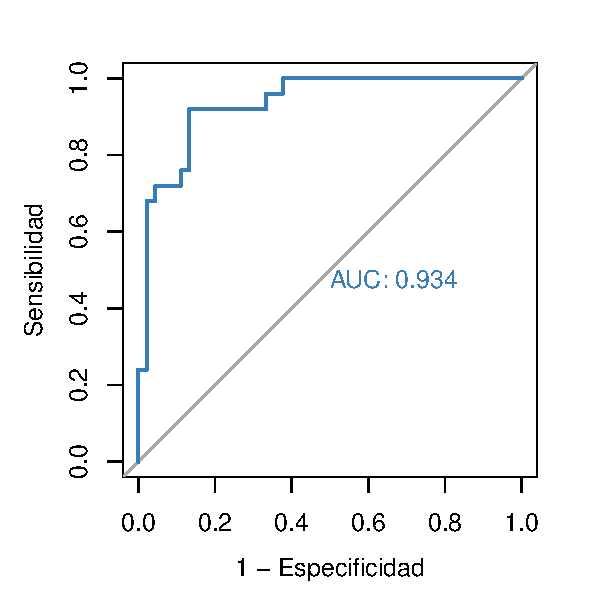
\includegraphics{Charaf-Spiousas_Clasificacion0_files/figure-latex/unnamed-chunk-11-1} 

}

\caption{\label{fig:roc}Curva ROC del modelo seleccionado con los datos de testeo.}\label{fig:unnamed-chunk-11}
\end{figure}

Para analizar el balance entre sensibilidad y especificidad del método
elegido, graficamos la curva ROC asociada (figura \ref{fig:roc}) y
calculamos el AUC cuyo valor es 0.929. Como el valor obtenido del AUC es
cercano a 1, podemos decir que el mecanismo de clasificación
seleccionado tiene un buen desempeño para distinguir entre las clases.

\hypertarget{anuxe1lisis-del-modelo-glm-usando-uxfanicamente-las-covariables-ck-y-h}{%
\subsubsection{Análisis del modelo GLM usando únicamente las covariables
CK y
H}\label{anuxe1lisis-del-modelo-glm-usando-uxfanicamente-las-covariables-ck-y-h}}

Como en el problema se indica que CK y H son más baratas de medir que PK
y LD, vamos a estudiar el modelo de regresión logística con
regularización LASSO considerando únicamente como variables predictoras
a CK y H.

Para eso, primero volvemos a explorar cuáles son los parámetros que
maximizan el promedio del F1 barriendo una grilla de valores de
\(\lambda\) y p y utilizando el método de validación cruzada, al igual
que lo realizado cuando teníamos las cuatro variables predictoras. El
valor máximo de F1 es 0.734 y se alcanza para \(p=\) 0.2 y \(\lambda=\)
0.039069.

Luego, ajustamos el modelo con los parámetros óptimos con toda la
muestra de entrenamiento y evaluamos sobre la muestra de testeo el F1
obteniendo un resultado de 0.769. El valor del error de clasificación
para los datos de testeo con dos variables es 0.171. La matriz de
confusión de este nuevo modelo es:

\begin{center}
\begin{tabular}{| c | c | c  c | }
\hline
& & \multicolumn{2}{ c| }{Verdaderos} \\ \hline
& & 0 & 1\\ \hline
Predichos & 0 & conf_2vars$table[1,1] & conf_2vars$table[1,2] \\
& 1 & conf_2vars$table[2,1] & conf_2vars$table[2,2] \\
 \hline
\end{tabular}
\end{center}

\hypertarget{conclusiones}{%
\subsection{Conclusiones}\label{conclusiones}}

En el trabajo exploramos distintos métodos para detectar la DMD y, en
base al análisis realizado, optamos por el modelo GLM con regularización
Lasso. Para tomar esta decisión nos basamos en que la métrica evaluada
dio considerablemente bien y el desempeño obtenido es similar al resto
de los métodos y nos permite tener una mayor interpretabilidad.

A la vez, indagamos sobre el impacto que tiene prescindir de las
variables PK y LD y, si bien se observa que las métricas empeoran un
poco, consideramos que si el costo de medición de las mismas es mucho
mayor se podría contemplar utilizar el modelo sin incluirlas.

Por último, en relación al dato sobre la probabilidad de que una mujer
sea portadora (1/3200), creemos que esta información podría ser
relevante en caso de que por algún motivo querramos tener un control
sobre la cantidad de falsos positivos (por ejemplo, si el paciente
tuviera que realizar un tratamiento costoso o de grande impacto en su
salud). Esto se debe a que al ser tan baja la probabilidad de que una
mujer sea portadora, la cantidad de falsos positivos será
considerablemente mayor que la cantidad de falsos negativos.

\end{document}
